% !TEX root = ../main.tex

% 结语部分
\section{APL1-3 氦氖激光综合实验 \\ The End}


%---------------------------------------------------------------------
% 总结、杂谈与致谢
\subsection{Summary, Thoughts \& Acknowledgments}
\begin{enumerate}
	\item \textbf{Summary:}本次氦氖激光综合实验围绕氦氖激光器的工作原理、光束特性及光学参数测量展开。实验分为多个环节,包括对激光器工作原理的预习、横模和纵模的概念理解、实验数据采集以及数据分析。通过实验操作,我们测量了光束通过透镜前后的光斑大小,并计算了光腰位置、光腰半径、远场发散角、瑞利长度等关键参数。实验结果显示,激光器直接输出的光束不具备理想的平行性,且在通过透镜后光腰位置并未完全位于透镜焦点,这一现象与高斯光束模型的实际特性相符。
	
	实验中的数据处理采用双曲线拟合和线性拟合相结合的方法,并使用了q参数矩阵变换的理论计算出不同状态下的光束参数。然而,由于光束质量和实验误差的影响,部分数据与理论值存在偏差。总体而言,实验验证了高斯光束模型及其传播特性,为理解氦氖激光器的工作机理提供了实践基础。
	
	\item \textbf{Thoughts:}如果可能,可以尝试优化激光器的腔内结构或使用更高质量的激光器,以获得接近理想的高斯光束输出,从而提高实验数据的精确度。引入更高精度的测量仪器,如精密定位台和高分辨率的测量工具,以减少实验数据的误差,特别是在光腰位置和光斑直径的测量上。在光束通过透镜后的测量位置上增加数据采样点,特别是靠近光腰处,以提高拟合精度,得到更准确的光束参数。利用编程进一步自动化数据分析过程,减少人为误差,并提高数据处理的效率和准确性。
	
	\item \textbf{Acknowledgments:}Thank you, teacher, for taking the time to read this experimental report, which still has many shortcomings. I hope you can point out the areas that need improvement. I wish you good health, happiness in life, and success in your work!
\end{enumerate}


%---------------------------------------------------------------------
% 附件
\subsection{Attachment}
%The arrangement of the experimental bench desktop is shown in %\cref{}.

The personal signature of the experimental report is shown in \cref{fig:name}.

\begin{figure}[H]
	\centering
	\begin{minipage}{0.3\textwidth}
		\centering
		
\includegraphics[width=\textwidth]{name.png}
		\caption{signature1}
		\label{fig:name}
	\end{minipage}
	\begin{minipage}{0.3\textwidth}
		\centering
		
\includegraphics[width=\textwidth]{images/name-TaLEs}
		\caption{signature2}
		\label{fig:name-tales}
	\end{minipage}
	% \begin{minipage}{0.3\textwidth}
	% 	\centering
	% 	\includegraphics[width=\textwidth]{images/name_mwc}
	% 	\caption{signature3}
	% 	\label{fig:namemwc}
	% \end{minipage}
	\begin{minipage}{0.25\textwidth}
		\centering
		% 使用\rotatebox命令逆时针旋转90度
		\rotatebox{90}{\includegraphics[width=\textwidth]{images/name_mwc}}
		\captionof{figure}{signature3}
		\label{fig:namemwc}
	\end{minipage}
	\begin{minipage}{0.3\textwidth}
		\centering
		\includegraphics[width=\textwidth]{images/name_zzx}
		\caption{signature3}
		\label{fig:namezzx}
	\end{minipage}
	
	\vspace{0.3cm} % 行距调整
	
	\begin{minipage}{0.3\textwidth}
		\centering
		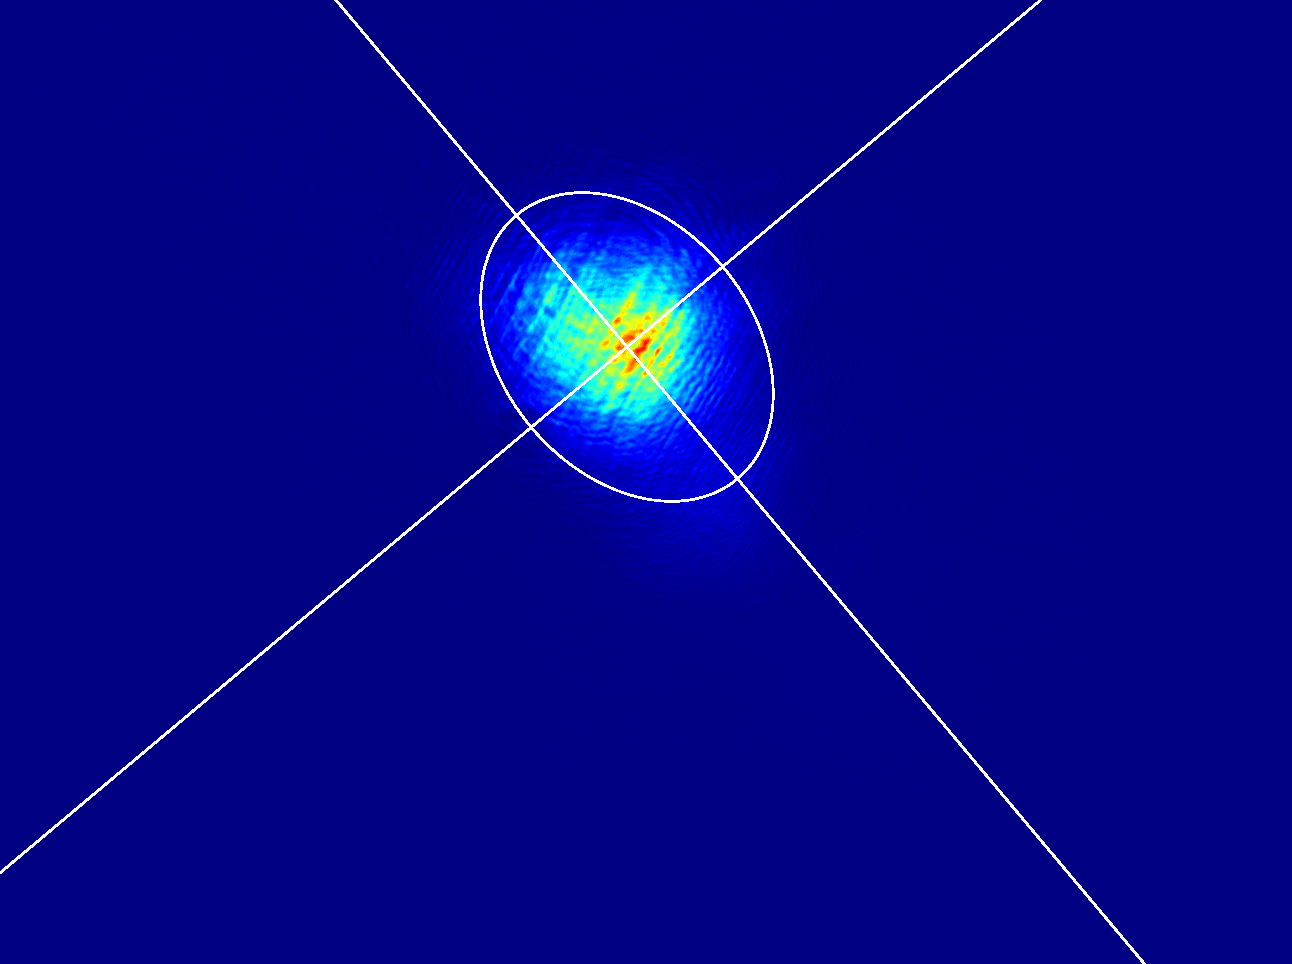
\includegraphics[width=\textwidth]{images/APL1_8_exp2_1_ccd}
		\caption{He-Ne单模CCD拍摄结果}
		\label{fig:apl18exp21ccd}
	\end{minipage}
	\begin{minipage}{0.3\textwidth}
		\centering
		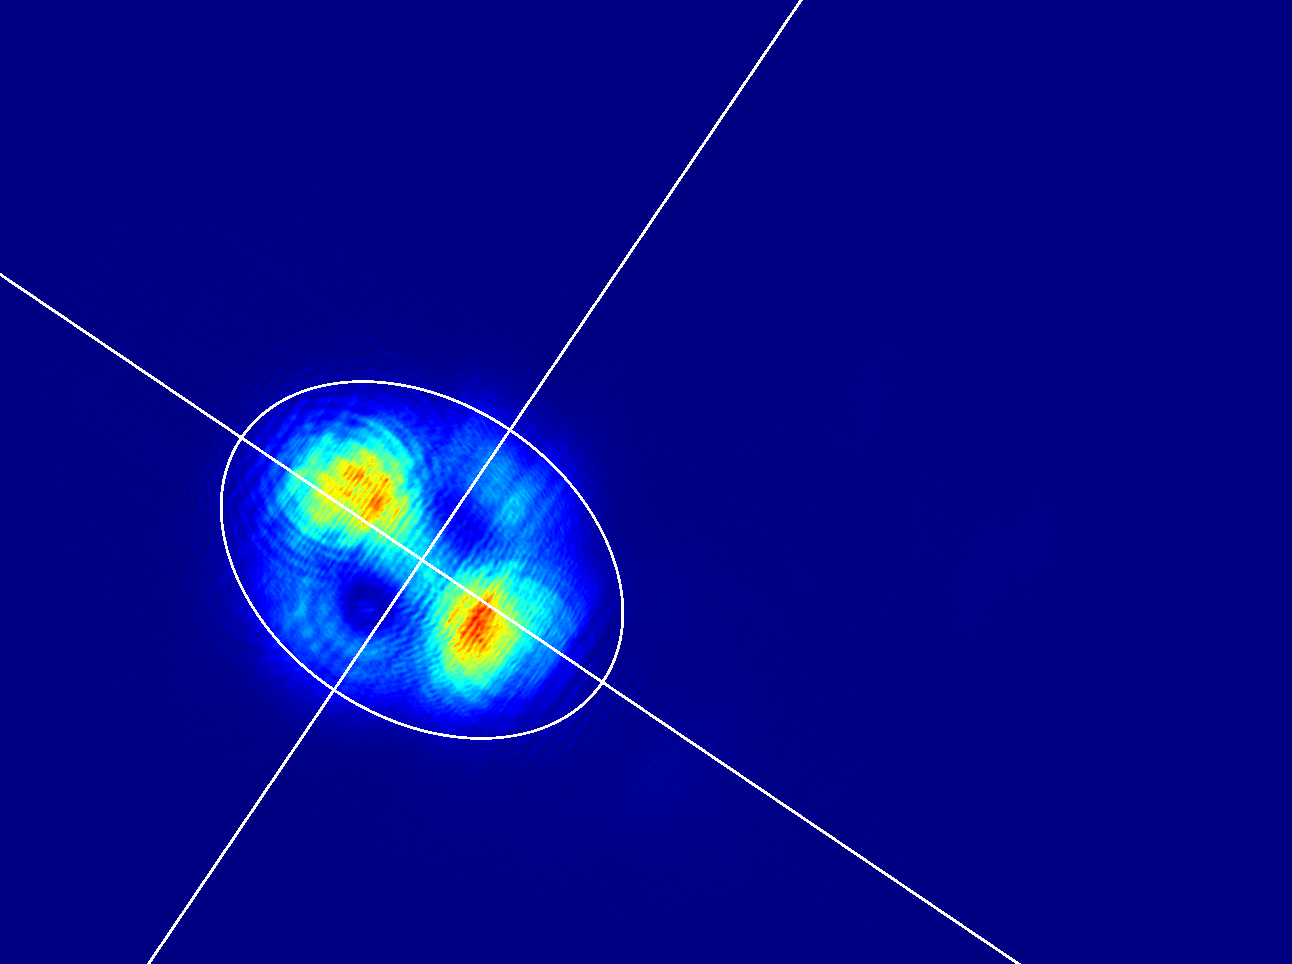
\includegraphics[width=\textwidth]{images/APL1_8_exp2_2_ccd}
		\caption{He-Ne混模CCD拍摄结果}
		\label{fig:apl18exp22ccd}
	\end{minipage}
	\begin{minipage}{0.3\textwidth}
		\centering
		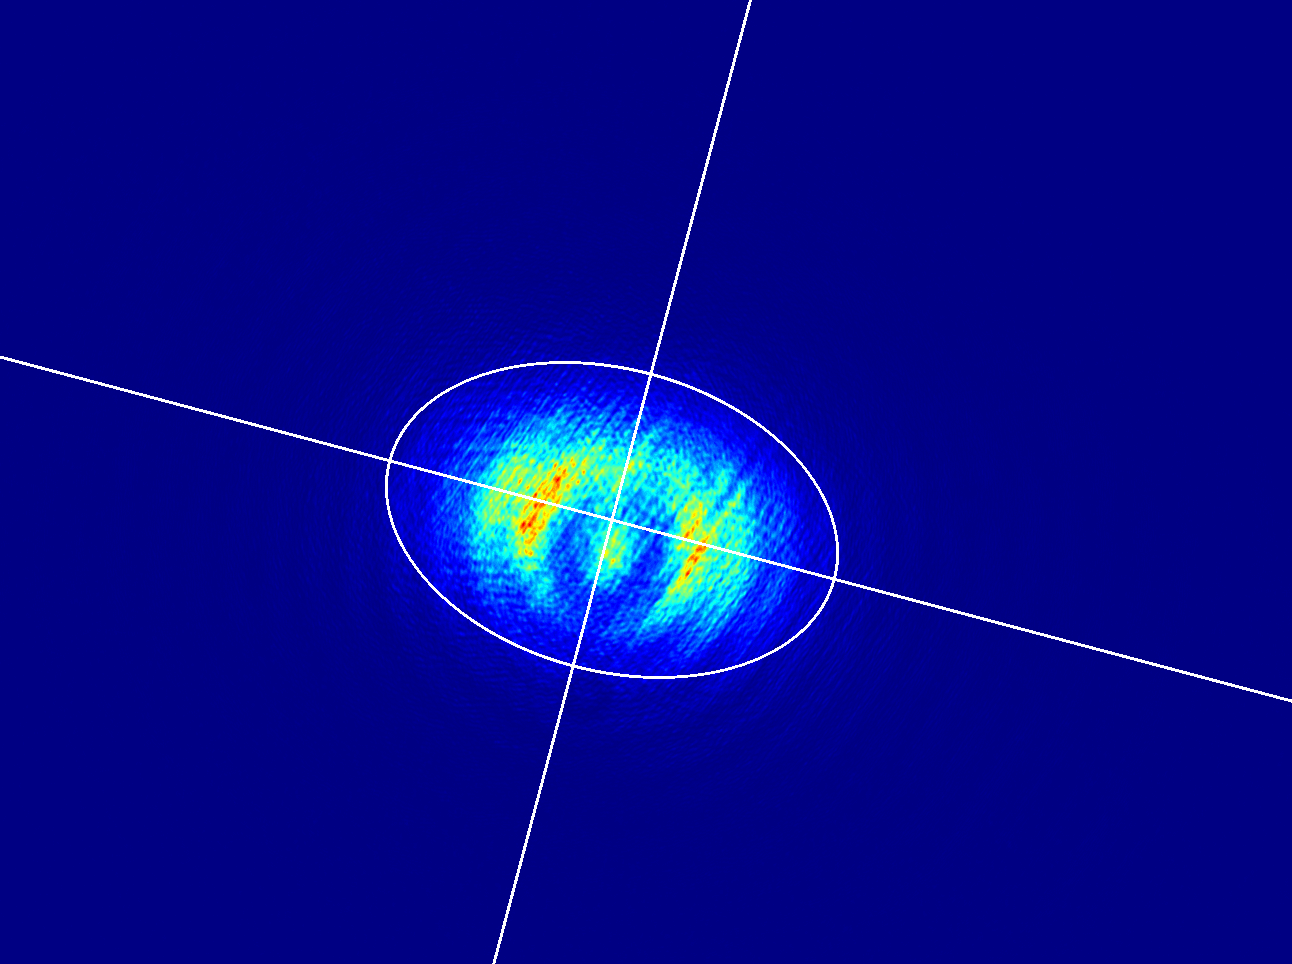
\includegraphics[width=\textwidth]{images/APL1_8_exp2_3_ccd}
		\caption{半导体混模CCD拍摄结果}
		\label{fig:apl18exp23ccd}
	\end{minipage}
	
	\vspace{0.3cm} % 行距调整
	
	\begin{minipage}{0.3\textwidth}
		\centering
		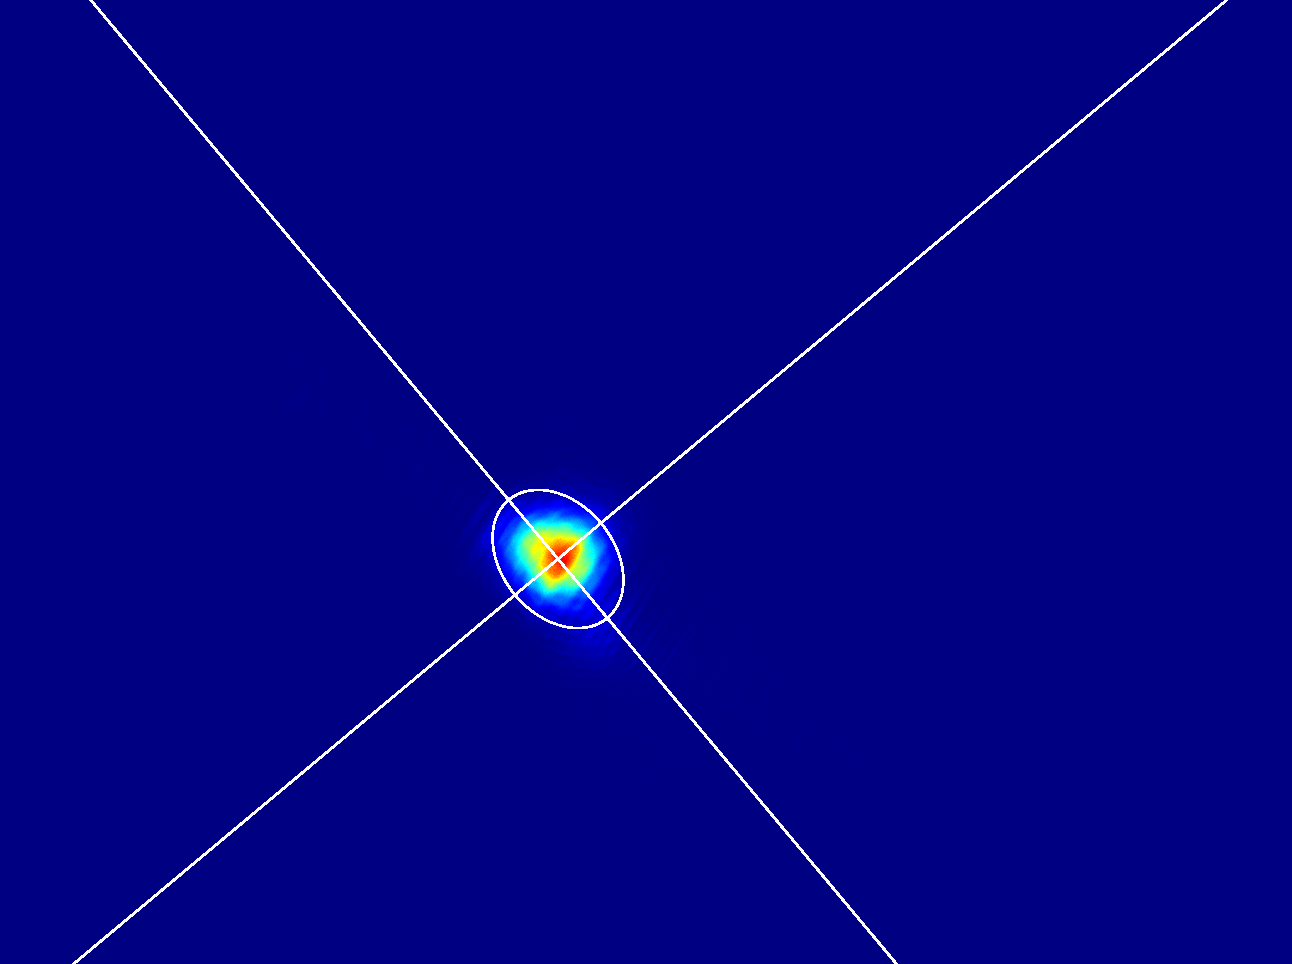
\includegraphics[width=\textwidth]{images/APL1_8_exp3_ccd}
		\caption{CCD拍摄结果}
		\label{fig:apl18exp3ccd}
	\end{minipage}
	\begin{minipage}{0.3\textwidth}
		\centering
		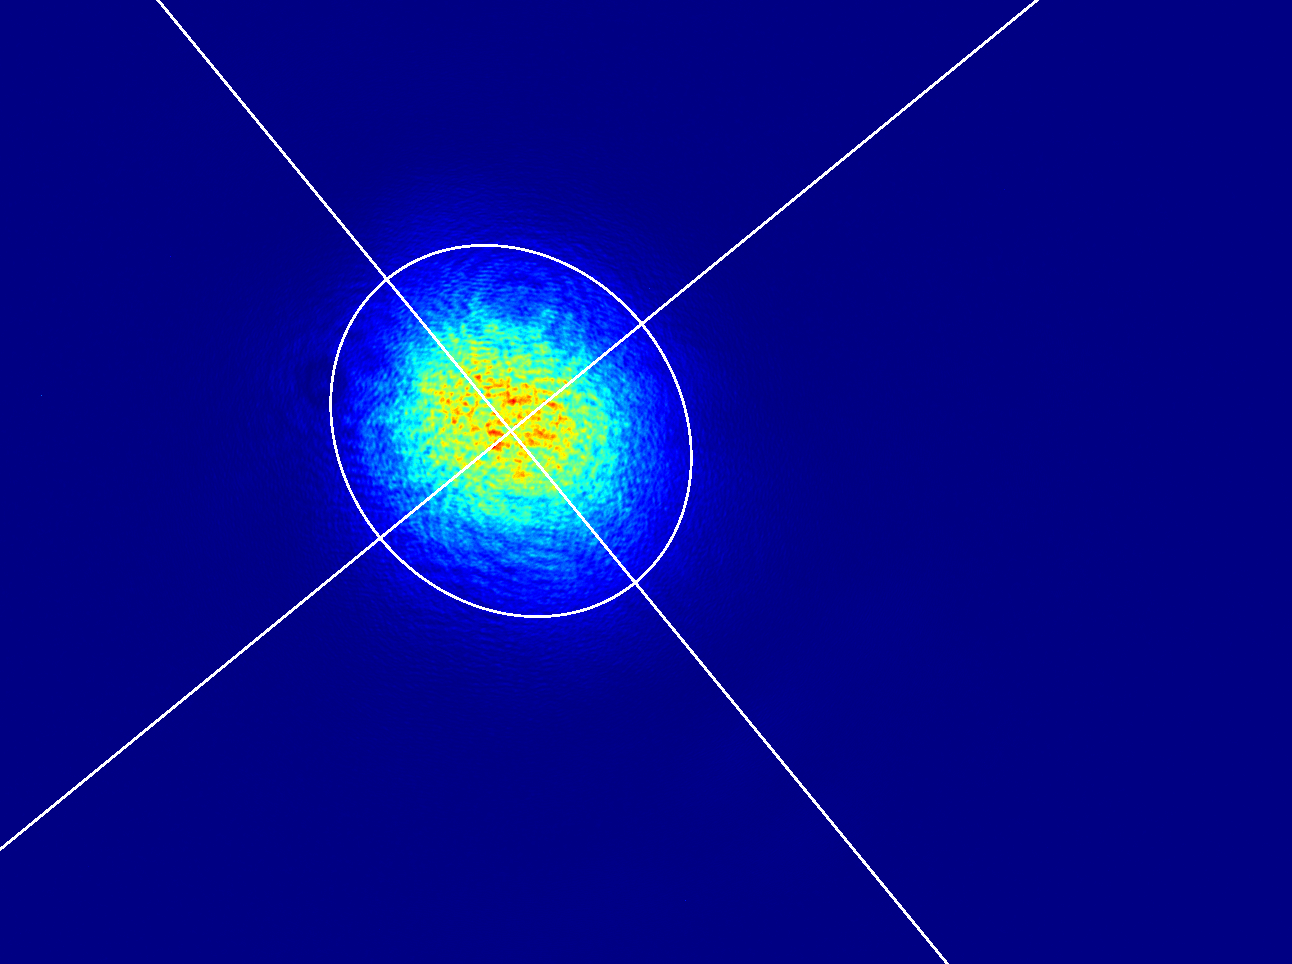
\includegraphics[width=\textwidth]{images/APL1_8_exp4_ccd}
		\caption{无透镜CCD拍摄结果}
		\label{fig:apl18exp4ccd}
	\end{minipage}
	\begin{minipage}{0.3\textwidth}
		\centering
		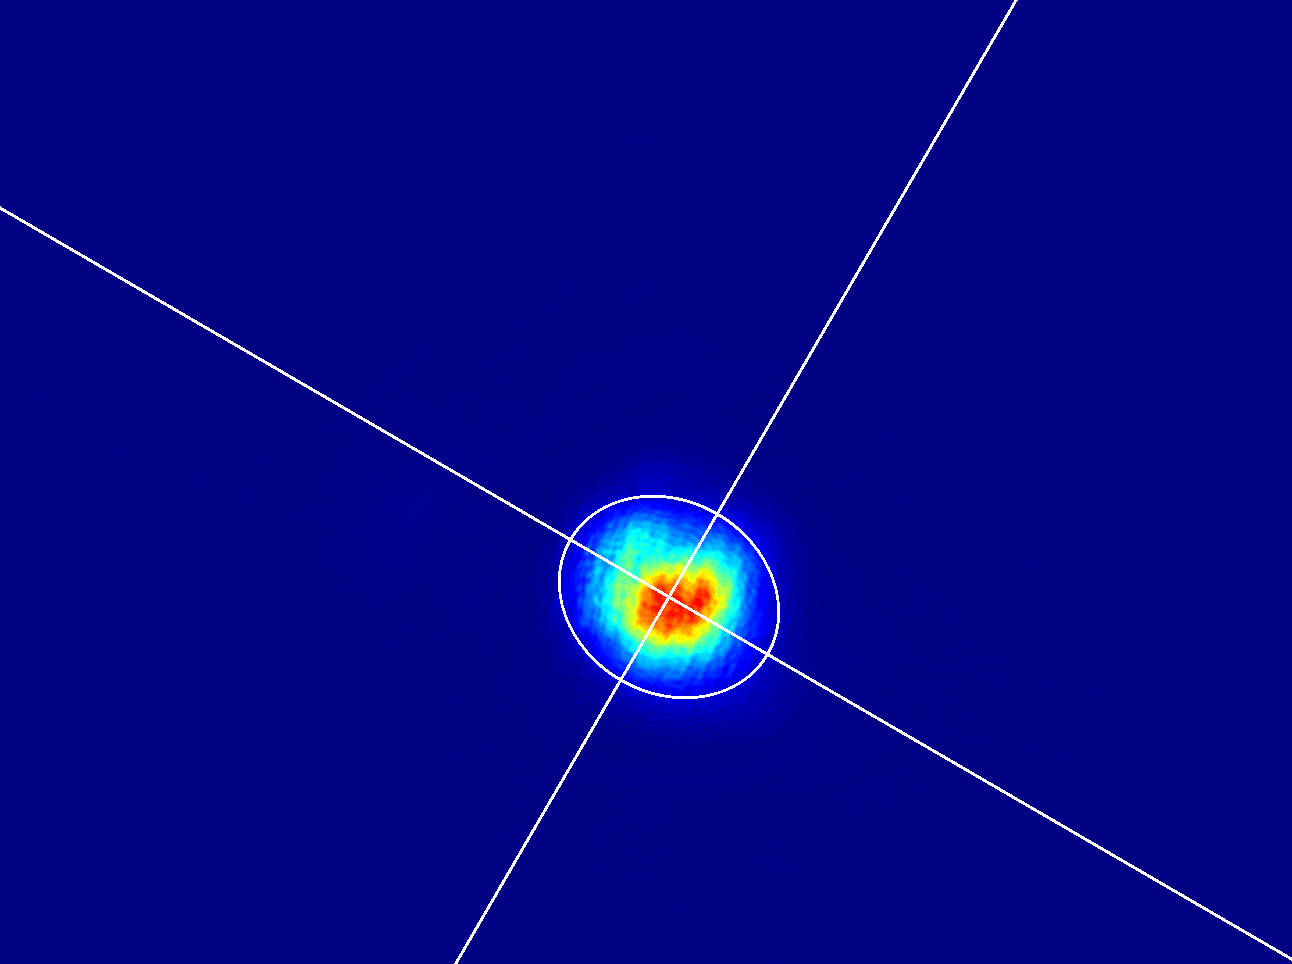
\includegraphics[width=\textwidth]{images/APL1_8_exp4_ccdT}
		\caption{加透镜CCD拍摄结果}
		\label{fig:apl18exp4ccdt}
	\end{minipage}
	
\end{figure}

\clearpage
\begin{lstlisting}[style=pythonstyle,caption=核心代码记录]
	# 读取数据
	file_path = "spot-parameter_lens.xlsx"
	data = pd.read_excel(file_path)
	z_positions = data['位置(mm)']  # 光束传播轴上的位置
	a_axis = data['a轴长(mm)']     # a 轴长(代表束宽)
	
	# 计算束宽,取 a 轴长和 b 轴长的平均值
	w_z = (data['a轴长(mm)'] + data['b轴长(mm)']) / 2
	
	# 定义双曲线拟合方程
	def hyperbolic_fit(z, A, B, C):
	return A + B * z + C * z**2
	
	# 拟合数据
	params, _ = curve_fit(hyperbolic_fit, z_positions, w_z**2)
	A, B, C = params
	
	# 计算光束参数
	z_0 = -B / (2 * C)                     # 光腰位置
	omega_0 = np.sqrt(A - B**2 / (4 * C))   # 光腰半径
	theta = np.sqrt(C)                      # 远场发散角
	Z_0 = (1 / (2 * C)) * np.sqrt(4 * A * C - B**2)  # 瑞利长度
	
	# 输出计算结果
	print(f"Beam Waist Position (z0): {z_0:.2f} mm")
	print(f"Beam Waist Radius (ω0): {omega_0:.4f} mm")
	print(f"Divergence Angle (θ): {theta:.6f} rad")
	print(f"Rayleigh Length (Z0): {Z_0:.2f} mm")
\end{lstlisting}

\clearpage
\begin{lstlisting}[style=pythonstyle,caption=其它计算代码]
	###
	
	# 读取数据
	file_path = "spot-parameter_lens.xlsx"
	data = pd.read_excel(file_path)
	z_positions = data['位置(mm)']  # 光束传播轴上的位置
	a_axis = data['a轴长(mm)']     # a 轴长(代表束宽)
	
	# 计算束宽,取 a 轴长和 b 轴长的平均值
	w_z = (data['a轴长(mm)'] + data['b轴长(mm)']) / 2
	
	# 定义双曲线拟合方程
	def hyperbolic_fit(z, A, B, C):
	return A + B * z + C * z**2
	
	# 拟合数据
	params, _ = curve_fit(hyperbolic_fit, z_positions, w_z**2)
	A, B, C = params
	
	# 计算光束参数
	z_0 = -B / (2 * C)                     # 光腰位置
	omega_0 = np.sqrt(A - B**2 / (4 * C))   # 光腰半径
	theta = np.sqrt(C)                      # 远场发散角
	Z_0 = (1 / (2 * C)) * np.sqrt(4 * A * C - B**2)  # 瑞利长度
	
	# 输出计算结果
	print(f"Beam Waist Position (z0): {z_0:.2f} mm")
	print(f"Beam Waist Radius (ω0): {omega_0:.4f} mm")
	print(f"Divergence Angle (θ): {theta:.6f} rad")
	print(f"Rayleigh Length (Z0): {Z_0:.2f} mm")
	
	###
	
	# 定义线性拟合函数
	def linear_fit(z, m, c):
	return m * z + c
	
	# 线性拟合
	params, covariance = curve_fit(linear_fit, z_positions, w_z)
	slope, intercept = params
	
	# 拟合结果和 R² 计算
	w_fitted_linear = linear_fit(z_positions, slope, intercept)
	residuals = w_z - w_fitted_linear
	ss_res = np.sum(residuals**2)
	ss_tot = np.sum((w_z - np.mean(w_z))**2)
	r_squared = 1 - (ss_res / ss_tot)
	mse = np.mean(residuals**2)
	
	# 输出拟合参数和评估结果
	print(f"Slope (m): {slope:.6f}")
	print(f"Intercept (c): {intercept:.6f}")
	print(f"R-squared: {r_squared:.4f}")
	print(f"Mean Squared Error (MSE): {mse:.6f}")
	
	###
	
	# 采用直线拟合结果估算高斯光束的参数
	
	# λ = 632.8 nm
	wavelength = 0.6328  # 微米
	
	# 斜率 m 由拟合结果获得
	theta = np.arctan(slope)  # 远场发散角
	omega_0 = -0.001 * wavelength / (np.pi * theta)  # 计算束腰半径
	z_R = 1000 * np.pi * omega_0**2 / wavelength   # 计算瑞利长度
	
	# 输出结果
	print(f"Beam Waist Radius (ω0): {omega_0:.4f} mm")
	print(f"Rayleigh Length (zR): {z_R:.4f} mm")
	
	# 远场发散角 theta 等于线性拟合的斜率
	theta = slope  # 斜率已从拟合中得到
	# 计算束腰位置 z_0
	z_0_1 = (omega_0 - intercept) / theta
	
	# 输出结果
	print(f"Beam Waist Position (z0): {z_0_1:.4f} mm")
	
	# 若仅从渐近线考虑
	z_0_2 = -intercept/slope
	print(f"Beam Waist Position (z0): {z_0_2:.4f} mm")
	
	###
	
	def q_parameter(z, z0, z_R):
	'''
	如果光束轴沿 z 方向,光束腰部位于 z0,瑞利区间为 z_R,则复光束参数可以等价表示为:
	q = (z - z0) + i * z_R
	'''
	return complex(z - z0, z_R)
	
	def q_parameter_transform(q_in, a=1, b=0, c=-1/200, d=1):
	'''
	元件矩阵:
	(a, b)
	(c, d)
	
	由变换得到的q2为:
	q2 = (a * q1 + b) / (c * q1 + d)
	'''
	return (a * q_in + b) / (c * q_in + d)
\end{lstlisting}

\textbf{All relevant code (Python and LaTex source code) has been uploaded to Github.}


%---------------------------------------------------------------------
% 附表
\clearpage
\subsection{Schedule}

\textbf{The following is a data recording table that may be used in the experiment.}

\begin{table}[h!]
	\centering
	\caption{【实验一】不同曲率后腔镜在不同位置的功率最大值记录表}
	\begin{tabular}{@{}cccc@{}}
		\toprule
		\textbf{后腔镜曲率} & \textbf{位置 1} & \textbf{位置 2} & \textbf{位置 3} \\ \midrule
		曲率 1 & \makebox[3cm][c]{\rule{0pt}{2ex}} & \makebox[3cm][c]{\rule{0pt}{2ex}} & \makebox[3cm][c]{\rule{0pt}{2ex}} \\ \hline
		曲率 2 & \makebox[3cm][c]{\rule{0pt}{2ex}} & \makebox[3cm][c]{\rule{0pt}{2ex}} & \makebox[3cm][c]{\rule{0pt}{2ex}} \\ \hline
		曲率 3 & \makebox[3cm][c]{\rule{0pt}{2ex}} & \makebox[3cm][c]{\rule{0pt}{2ex}} & \makebox[3cm][c]{\rule{0pt}{2ex}} \\ \bottomrule
	\end{tabular}
\end{table}

\textbf{Recorder \& Time :}

\begin{table}[h]
	\centering
	\renewcommand{\arraystretch}{1.5} % 调整表格行高
	\caption{【实验2-1】单模激光光斑宽度的测量\quad 单位:(mm)}
	\begin{tabular}{|c|*{7}{p{1.7cm}|}}
		\hline
		\textbf{测量位置} & & & & & & & \\ \hline
		\textbf{水平宽度} & & & & & & & \\ \hline
		\textbf{垂直宽度} & & & & & & & \\ \hline
	\end{tabular}
\end{table}

\textbf{Recorder \& Time :}

\begin{table}[h]
	\centering
	\renewcommand{\arraystretch}{1.5} % 调整表格行高
	\caption{【实验2-2】多模激光光斑宽度的测量\quad 单位:(mm)}
	\begin{tabular}{|c|*{7}{p{1.7cm}|}}
		\hline
		\textbf{测量位置} & & & & & & & \\ \hline
		\textbf{水平宽度} & & & & & & & \\ \hline
		\textbf{垂直宽度} & & & & & & & \\ \hline
	\end{tabular}
\end{table}

\textbf{Recorder \& Time :}


%---------------------------------------------------------------------
% 参考文献
\clearpage
\renewcommand{\refname}{Reference}
\begin{thebibliography}{99}	
	\bibitem{a} 维基百科. \emph{维基百科}[M]. https://zh.wikipedia.org
	\bibitem{b} 沈韩. \emph{基础物理实验}[M]. 北京: 科学出版社, 2015.	
	\bibitem{svelto153} Svelto, O. \textit{Principles of Lasers}, 5th ed., Springer, 2010, p. 153.
	\bibitem{gouy_phase_shift} Siegman, A.E. \textit{Lasers}, University Science Books, 1986, p. 630.
	\bibitem{Brorson} S.D. Brorson, ``What is the confocal parameter?,'' \textit{IEEE Journal of Quantum Electronics}, vol. 24, no. 3, pp. 512–515, 1988. DOI: \texttt{10.1109/3.155}.
	\bibitem{Siegman1986} A.E. Siegman, \textit{Lasers}, University Science Books, 1986, p. 645.
	\bibitem{Paschotta2014} Rüdiger Paschotta, ``Gouy Phase Shift,'' \textit{Encyclopedia of Laser Physics and Technology}, RP Photonics, accessed May 2, 2014.
	\bibitem{siegman638} A.E. Siegman, \textit{Lasers}, University Science Books, 1986, pp. 638–640.
	\bibitem{garg168} Garg, K. \textit{Classical Optics and Its Applications}, Cambridge University Press, 2011, pp. 165–168.
	\bibitem{Rashidian2013} Rashidian Vaziri, M., Hajiesmaeilbaigi, F., Maleki, M. (2013). ``Propagation of Gaussian beams through optical systems''. 
	\bibitem{Lei} C. Tim Lei, \textit{Physics 4510 Optics webpage}, University of Colorado, 2024. \url{http://www.colorado.edu/physics/phys4510/phys4510_fa05/}.
\end{thebibliography}